\section{Simulation}\label{sec:experiments}
We present examples of maneuvering across diverse environments in a Gazebo simulation to demonstrate the framework's efficacy, scalability, and generalizability.
In addition, benchmarking experiments are conducted to further compare our proposed framework with pure-MIP approaches.

\revised{\subsection{Implementation Details}\label{sec:impl_details}
All MICP problems---including the offline gait-free MICP, the online gait-fixed MICP, the kinematic-feasibility re-targeting MICP, and the pure-MIP benchmark---are solved using Gurobi~9~\citep{gurobi}. The NMPC tracker is implemented with the OCS2 library~\citep{OCS2}. All offline-synthesis, simulation, and online-planning experiments are run on a desktop workstation equipped with an Intel Core i9-13900K (24 cores) and 64\,GB of RAM. Reported solve times reflect this desktop-class CPU and should be interpreted as such; onboard, low-power deployment is left as future work.}

\subsection{Robot Setup}
As shown in Fig.~\ref{fig:hardware_info}, we verify our algorithms on two separate robot platforms, Unitree Go2 and SkyMul Chotu (a modified Unitree Go1 robot dedicated for rebar tying tasks). The SkyMul Chotu is equipped with a rebar gun mounted on its head and customized ``cross"-shaped feet designed for reliable standing on rebars. Note that in simulation, this foot shape is simplified to a regular round foot to avoid the complexity of simulating contact with irregular surfaces. In our planner, we model both cases as point contact.
The parameters for each robot are defined in Table~\ref{tab:robot_parameter} and used in our implementation, including the robot mass $m$, torque limit $\vg \tau_{\text{max}}$ and the reference joint position $\v q_j^{\text{ref}}$ for a single leg with three joints, the reference foot position relative to the base frame $^\mathcal{B} \v p_j^{\text{ref}}$ and the maximum deviation of the foot position $\v p_j^{\text{max}}$ for the front left leg ($j=0$), and the moment of inertia of the approximated single rigid body $\v I$.
\begin{figure}[t]
    \centering
    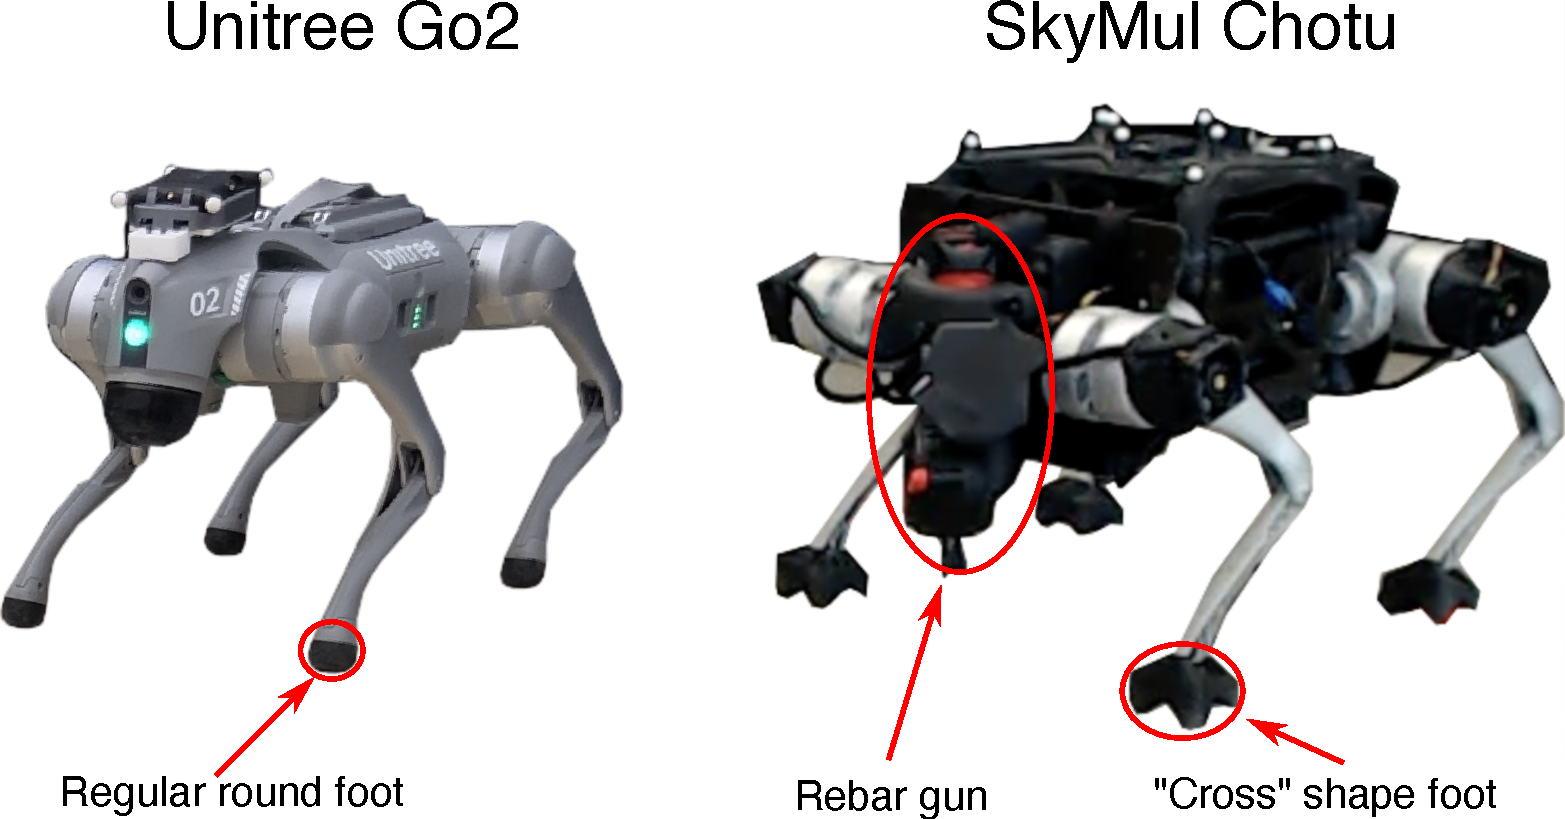
\includegraphics[width=0.85\linewidth]{hardware_info.pdf}
    \caption{Hardware platforms used for experiments: Unitree Go2 and SkyMul Chotu (equipped with a rebar gun and ``cross"-shaped feet).}
    \label{fig:hardware_info}
\end{figure}
\begin{table}[t]
\centering
\footnotesize
    \caption{Robot Parameters}
    \setlength{\tabcolsep}{4pt}
     \begin{tabular*}{\linewidth}{@{\extracolsep{\fill}}lll}
         \hline
         \textbf{Parameter} & \textbf{Unitree Go2} & \textbf{SkyMul Chotu}\\\hline
         $m$ (kg) & 15 & 20\\
         $\vg \tau_{\text{max}} $ (N $\cdot$ m) & (23.5, 23.5, 45.4) & (23.5, 23.5, 33.5)\\
         $\v q_j^{\text{ref}}$ (rad) & (0.0, 0.72, -1.44) & (0.0, 0.72, -1.44)\\
         $^\mathcal{B} \v p_j^{\text{ref}}$ (m) & (0.1805, 0.1308, -0.29) & (0.2118, 0.210, -0.30)\\
         $\v p_j^{\text{max}}$ (m) & (0.15, 0.1, 0.15) & (0.15, 0.1, 0.15)\\
         $\v I$ (kg $\cdot$ m$^2$) & diag(0.152, 0.369, 0.388) & diag(0.396, 0.915, 1.107)\\
         \hline
    \end{tabular*}
    \label{tab:robot_parameter}
\end{table}

% \todo Show the successful rate of navigation

\begin{figure*}[t!]
    \centering
    \includegraphics[width=\linewidth]{unstructured_and_rebar_maneuver_large.png}
    \caption{Snapshots from online execution across the four simulation scenarios: (a) unstructured terrain with four terrain types, (b) unstructured terrain with the full eight-type abstraction, (c) rebar terrain with the 7-type abstraction, and (d) rebar terrain with the 14-type abstraction. Green trajectories in (c) and (d) are detours produced by runtime re-synthesis after online MICP solving failures.}
    \label{fig:online_terrains}
\end{figure*}

\begin{table*}[t]
\centering
\footnotesize
    \caption{Offline Synthesis and Repair Time}
    \setlength{\tabcolsep}{4pt}
     \begin{tabular*}{\linewidth}{@{\extracolsep{\fill}}cccccc}
         \hline
         \textbf{Scenario} & \textbf{Grid Size} &
         % Terrain States $\times$ Request States
         \begin{tabular}{@{}c@{}}\textbf{Terrain and Request State Pairs}\\ \textbf{(Success/Total)}\end{tabular}
         & \begin{tabular}{@{}c@{}}\textbf{Number of Skills} \\ \textbf{(Original/New/Total)}\end{tabular} & \textbf{Symbolic Repair Time (s)} & \begin{tabular}{@{}c@{}}\textbf{Feasibility Check Time (s)}\\ \textbf{(Gait-Fixed/Gait-Free)}\end{tabular}\\\hline
         Unstructured - 4 & $3 \times 3$ & 169/169 & 18/\textcolor{red}{13}/64 & 8.07 &  18.97/449.94 \\
         & $5 \times 5$ & 129/158 & 19/\textcolor{red}{9}/64 & 77.16 &  20.26/241.42 \\\hline
         Unstructured - 8 & $3 \times 3$ & 250/264 & 19/\textcolor{red}{20}/256 & 14.90 & 22.92/382.63 \\
         & $5 \times 5$ & 179/246 & 20/\textcolor{red}{16}/256 & 93.21 & 18.59/196.88\\\hline
         Rebar - 7& $3 \times 3$ & 
         % -/258 & 47/-/52 & - &  116.69/- 
         196/196 & 18/\textcolor{red}{11}/196 & 7.44 &  15.63/417.55
         \\
         & $5 \times 5$ & 196/196 & 18/\textcolor{red}{10}/196 & 21.63 &  14.83/374.89 \\\hline
         Rebar - 14 & $3 \times 3$ & 237/237 & 20/\textcolor{red}{29}/784 & 10.34 & 21.92/701.38\\
         & $5 \times 5$ & 196/196 & 20/\textcolor{red}{18}/784 & 24.31 & 23.06/453.94 \\\hline
    \end{tabular*}
    \label{tab:offline_synthesis_time}
\end{table*}

\subsection{Simulation Environment Setup}
To demonstrate the generalizability of our proposed framework, we evaluate it across two scenarios involving different terrain types, safe stepping regions, and robotic platforms—Unitree Go2 and SkyMul Chotu. Obstacles are modeled as a distinct terrain class, and obstacle avoidance is encoded as hard constraints within $\syssafety$. The requested waypoints are assumed to be free of obstacles.
We test both $3 \times 3$ and $5 \times 5$ grid abstractions. The $5 \times 5$ grid enables a longer planning horizon but introduces higher decision complexity. For discretization, we use a cell size of 0.8 m in unstructured terrains and 0.6 m for the rebar case. These values can be adjusted based on the requirements of specific deployment environments.

% \begin{figure}[h]
%     \centering
%     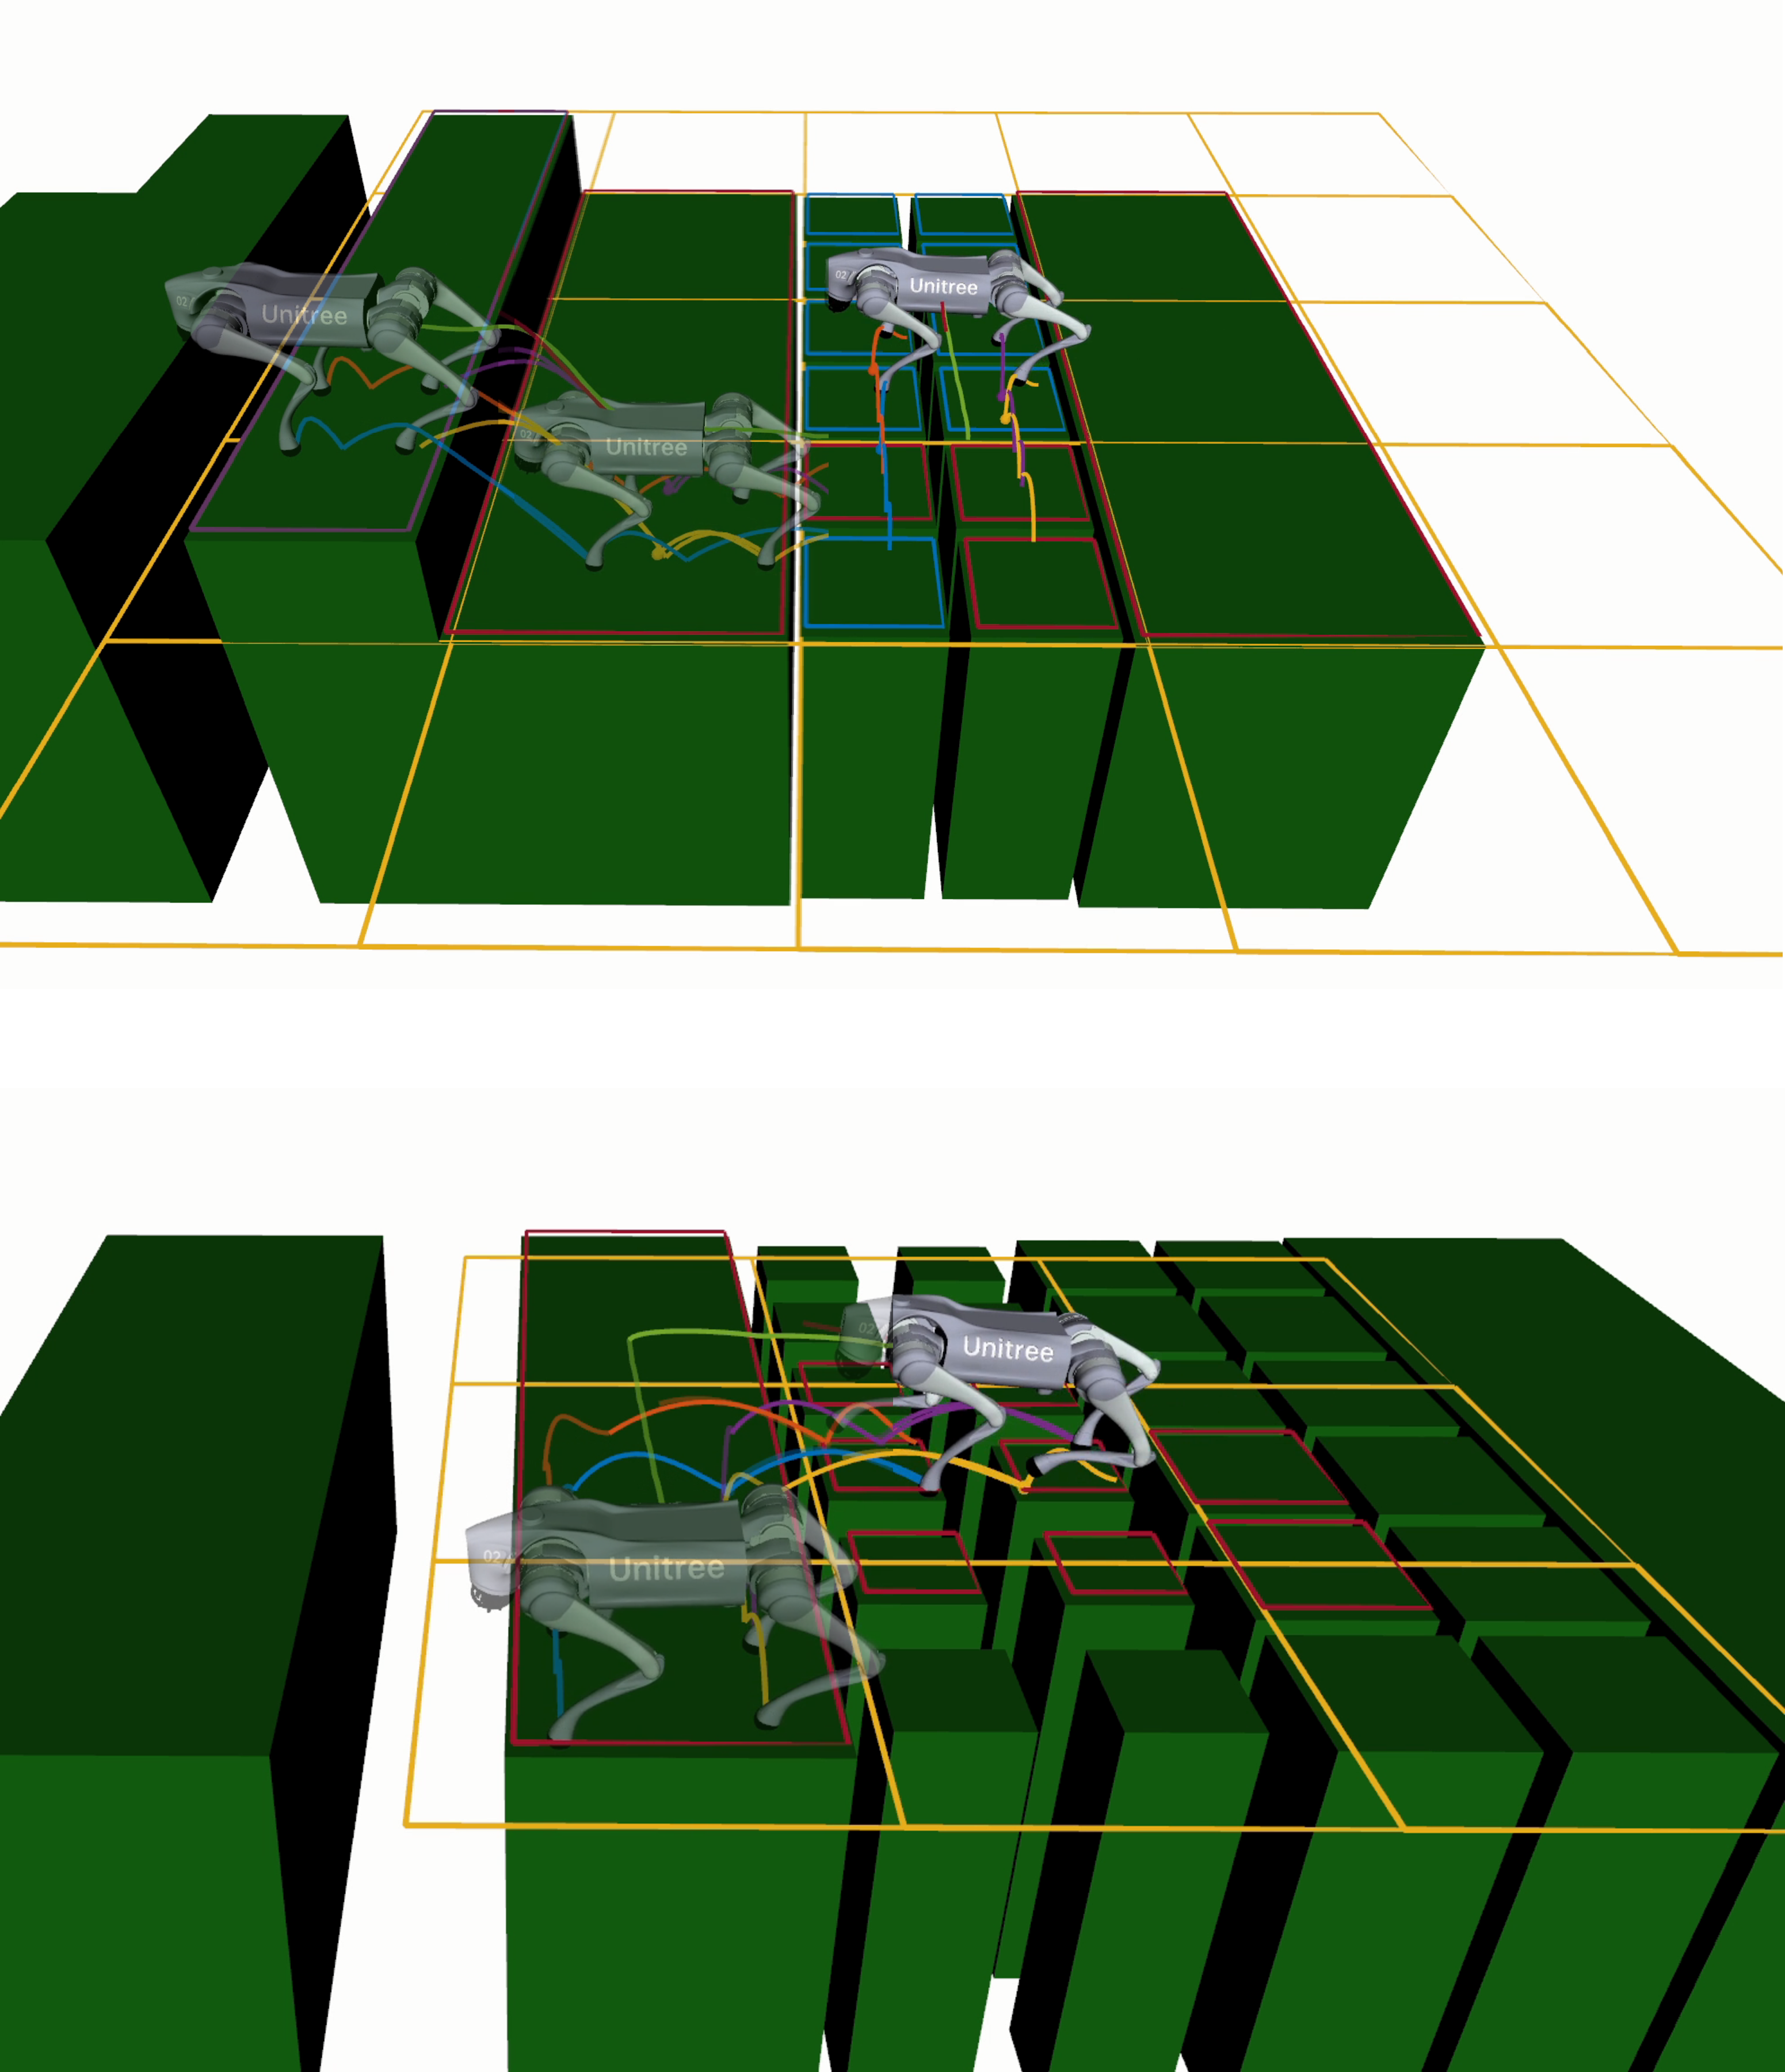
\includegraphics[width=\linewidth]{5x5_unstructured_demonstration.pdf}
%     \caption{Caption}
%     \label{fig:multiple_sizes}
% \end{figure}

\subsubsection{Unstructured Terrain}
% \begin{figure}
%     \centering
%     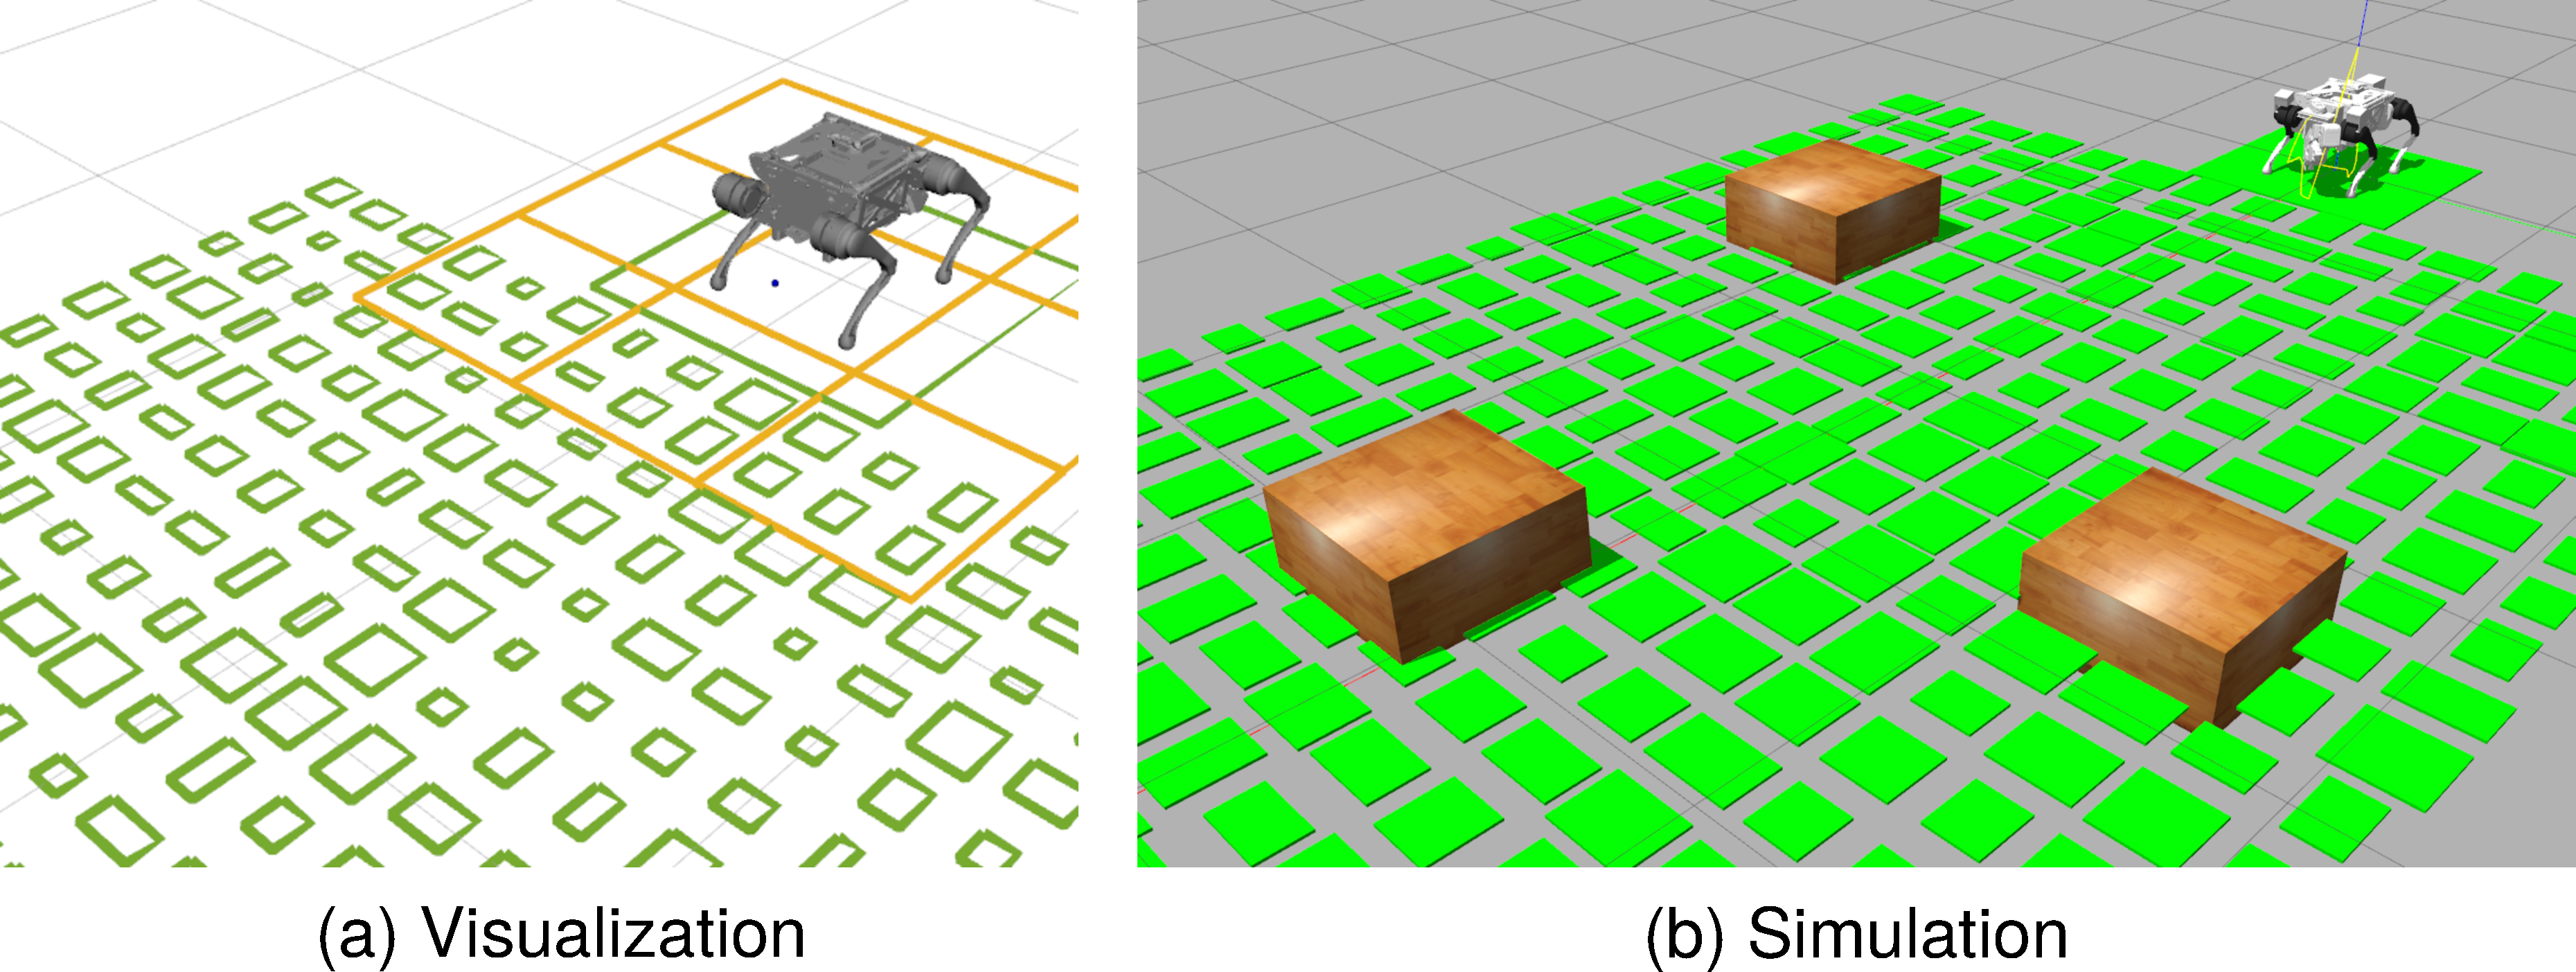
\includegraphics[width=\linewidth]{online_terrains.pdf}
%     \caption{(Will be updated to have rebar scenario.) Online scenarios with random sparsity of stepping stone and obstacles.}
%     \label{fig:online_terrains}
% \end{figure}
% Unlike Example \ref{example:1}, to further study the scalability of the proposed framework, 
We abstract 8 terrain types—\textit{flat terrain}, \textit{high terrain}, \textit{low terrain}, \textit{dense stone}, \textit{sparse stone}, \textit{gap}, \textit{high gap}, and \textit{low gap}—based on classification criteria involving polygon heights, counts, and areas relative to the abstracted grid cells. A terrain is categorized as a \textit{gap} when the ratio of its overlapping area with a grid cell falls below a specified threshold.
We define two terrain configurations: one consisting of four selected terrain types, and another comprising all eight. These are illustrated in Figs.~\ref{fig:online_terrains}(a) and \ref{fig:online_terrains}(b), respectively.
% \begin{figure}[h]
%     \centering
%     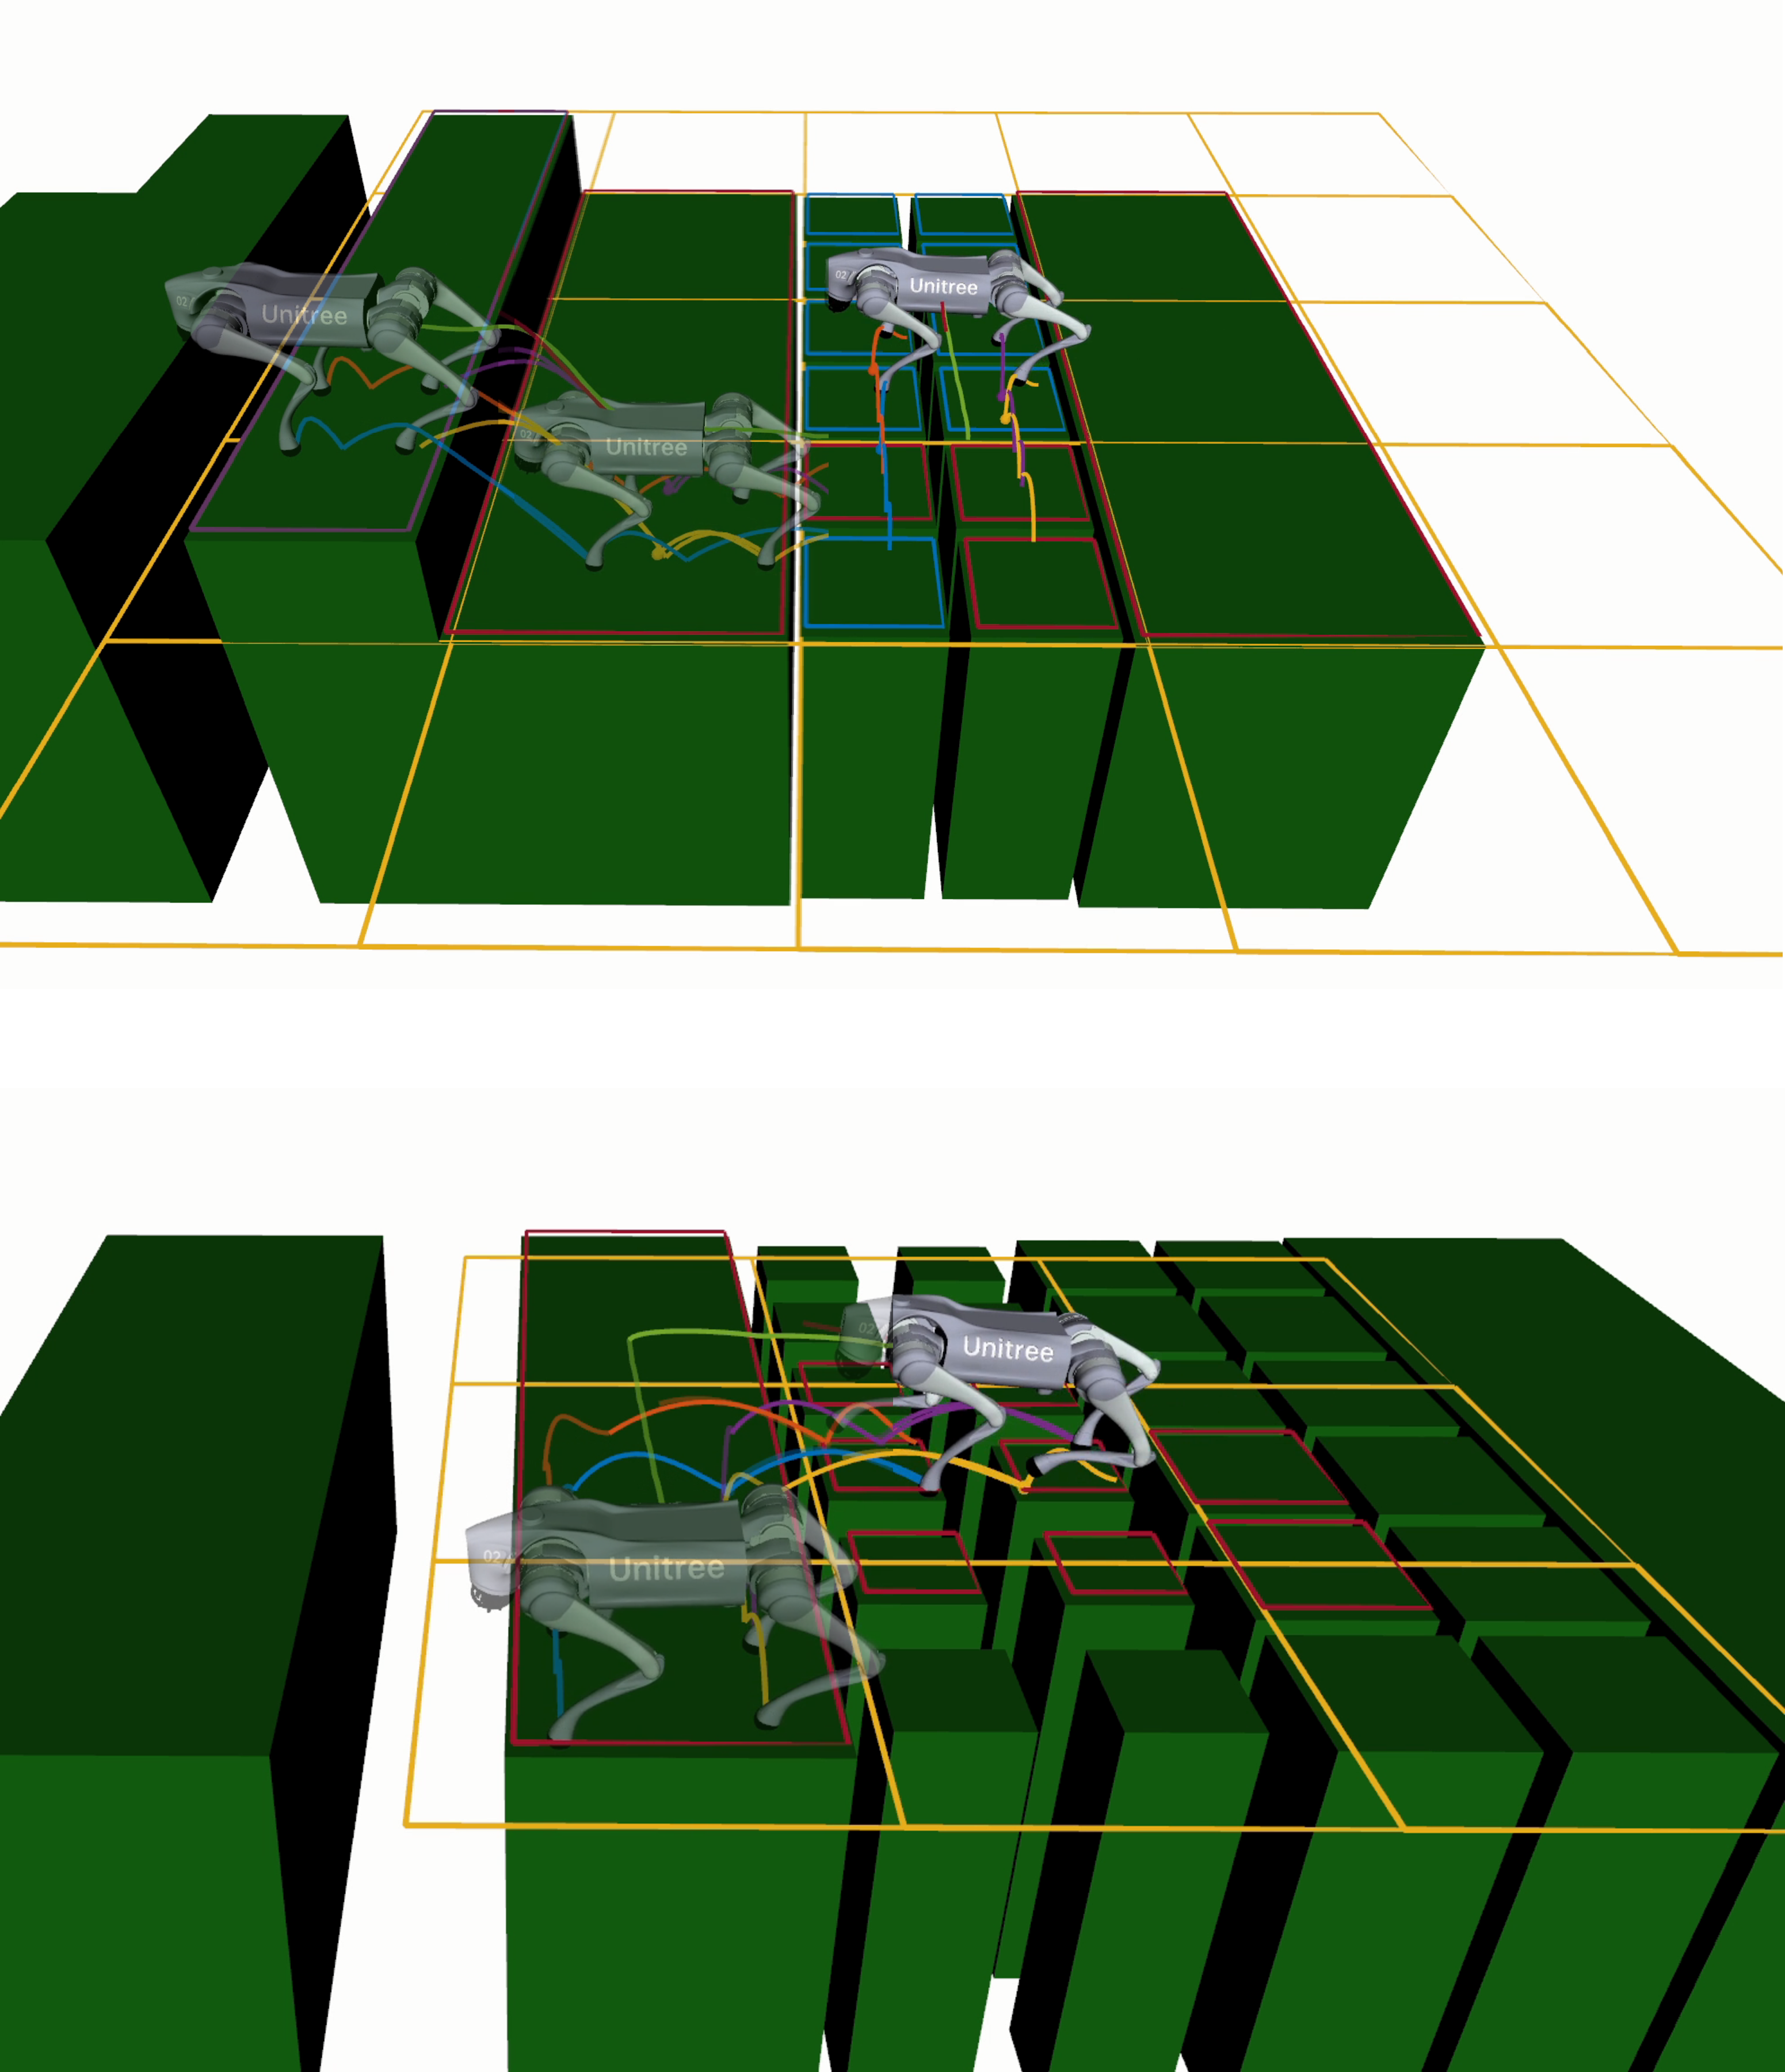
\includegraphics[width=\linewidth]{5x5_unstructured_demonstration.pdf}
%     \caption{Local environment abstraction and maneuvering with 5x5 (upper) and 3x3 (lower) grid size in separate unstructured terrain scenarios.}
%     \label{fig:multiple_sizes}
% \end{figure}

\subsubsection{Rebar Terrain}
% Inspired by automating labor-intensive rebar tying tasks on construction sites \citep{asselmeier2024hierarchical}, we explore a second case study where the quadrupedal robot navigates a rebar mat. 
% We model each rebar as a rectangular polygon with a 3 cm width. 
% Unlike the stepping stone scenario, this setup offers a larger number of potential stepping polygons due to the higher rebar density. 
% Observing that the robot's traversability depends on rebar sparsity in different directions—whether aligned with the robot's facing direction or not, 
% within a given tolerance—we abstract and classify rebar types based on a combination of horizontal sparsity (perpendicular to the robot's facing direction) and vertical sparsity (parallel to it). 
% %
% By calculating the number and relative spacing of the rebars inside each abstracted cell, we categorize each direction's sparsity as  \textit{dense} (0.05 - 0.15 m), \textit{sparse} (0.15 - 0.35 m), or \textit{extreme sparse} (above 0.35 m), \textit{single}, \textit{none}. 
% To reduce the complexity of the problem, we remove some challenging combinations such as \textit{none} or \textit{single} in both directions and treat them as \textit{obstacle}. As a result, we define two example configurations with 7 and 14 rebar terrain types. The 7-type scenario in Fig.~\ref{fig:online_terrains}(c) generates random rebar sparsity between 0.15 and 0.35 m, excluding the \textit{extreme sparse} type. In contrast, the 14-type scenario in Fig.~\ref{fig:online_terrains}(d)  includes rebar sparsity from 0.15 to 0.6 m, potentially covering more challenging combinations including the \textit{extreme sparse} ones.
Inspired by efforts to automate labor-intensive rebar tying tasks on construction sites \citep{asselmeier2024hierarchical}, we investigate a second case study in which a quadrupedal robot navigates a rebar mat. Each rebar is modeled as a rectangular polygon with a 3 cm width. Unlike the stepping stone scenario, this setup presents a denser distribution of potential footholds due to the higher rebar density. Notably, the robot’s traversability depends on the directional sparsity of the rebars—whether aligned with or orthogonal to the robot’s facing direction—within an acceptable tolerance.

We abstract and classify rebar types based on horizontal sparsity (perpendicular to the robot’s facing direction) and vertical sparsity (parallel to it). Within each abstracted cell, the number and spacing of rebars are evaluated to classify the sparsity in each direction as \textit{dense} (0.05–0.15 m), \textit{sparse} (0.15–0.35 m), \textit{extreme sparse} (above 0.35 m), \textit{single}, or \textit{none}. To reduce complexity, combinations deemed too challenging—such as \textit{none} or \textit{single} in both directions—are treated as \textit{obstacle}.
Based on this abstraction, we define two example configurations comprising 7 and 14 rebar terrain types. The 7-type configuration in Fig.~\ref{fig:online_terrains}(c) samples rebar sparsity randomly between 0.15 and 0.35 m, omitting \textit{extreme sparse} regions. In contrast, the 14-type configuration in Fig.~\ref{fig:online_terrains}(d) includes sparsity ranging from 0.15 to 0.6 m, encompassing more complex and difficult combinations including \textit{extreme sparse} types.
\begin{figure*}[t]
    \centering
    \includegraphics[width=\linewidth]{online_repair_new_gap.pdf}
    \caption{Runtime symbolic repair triggered by an unforeseen \textit{gap} state in the \textit{Unstructured-4} / $3\times 3$ scenario, in which gap states are deliberately excluded offline. Repair proposes the missing transition and gait-free MICP synthesizes a leaping skill, taking $12.36$\,s total ($0.18$\,s symbolic repair + $12.18$\,s gait-free MICP).}
    \label{fig:online_repair}
\end{figure*}

\begin{figure}[t]
    \centering
    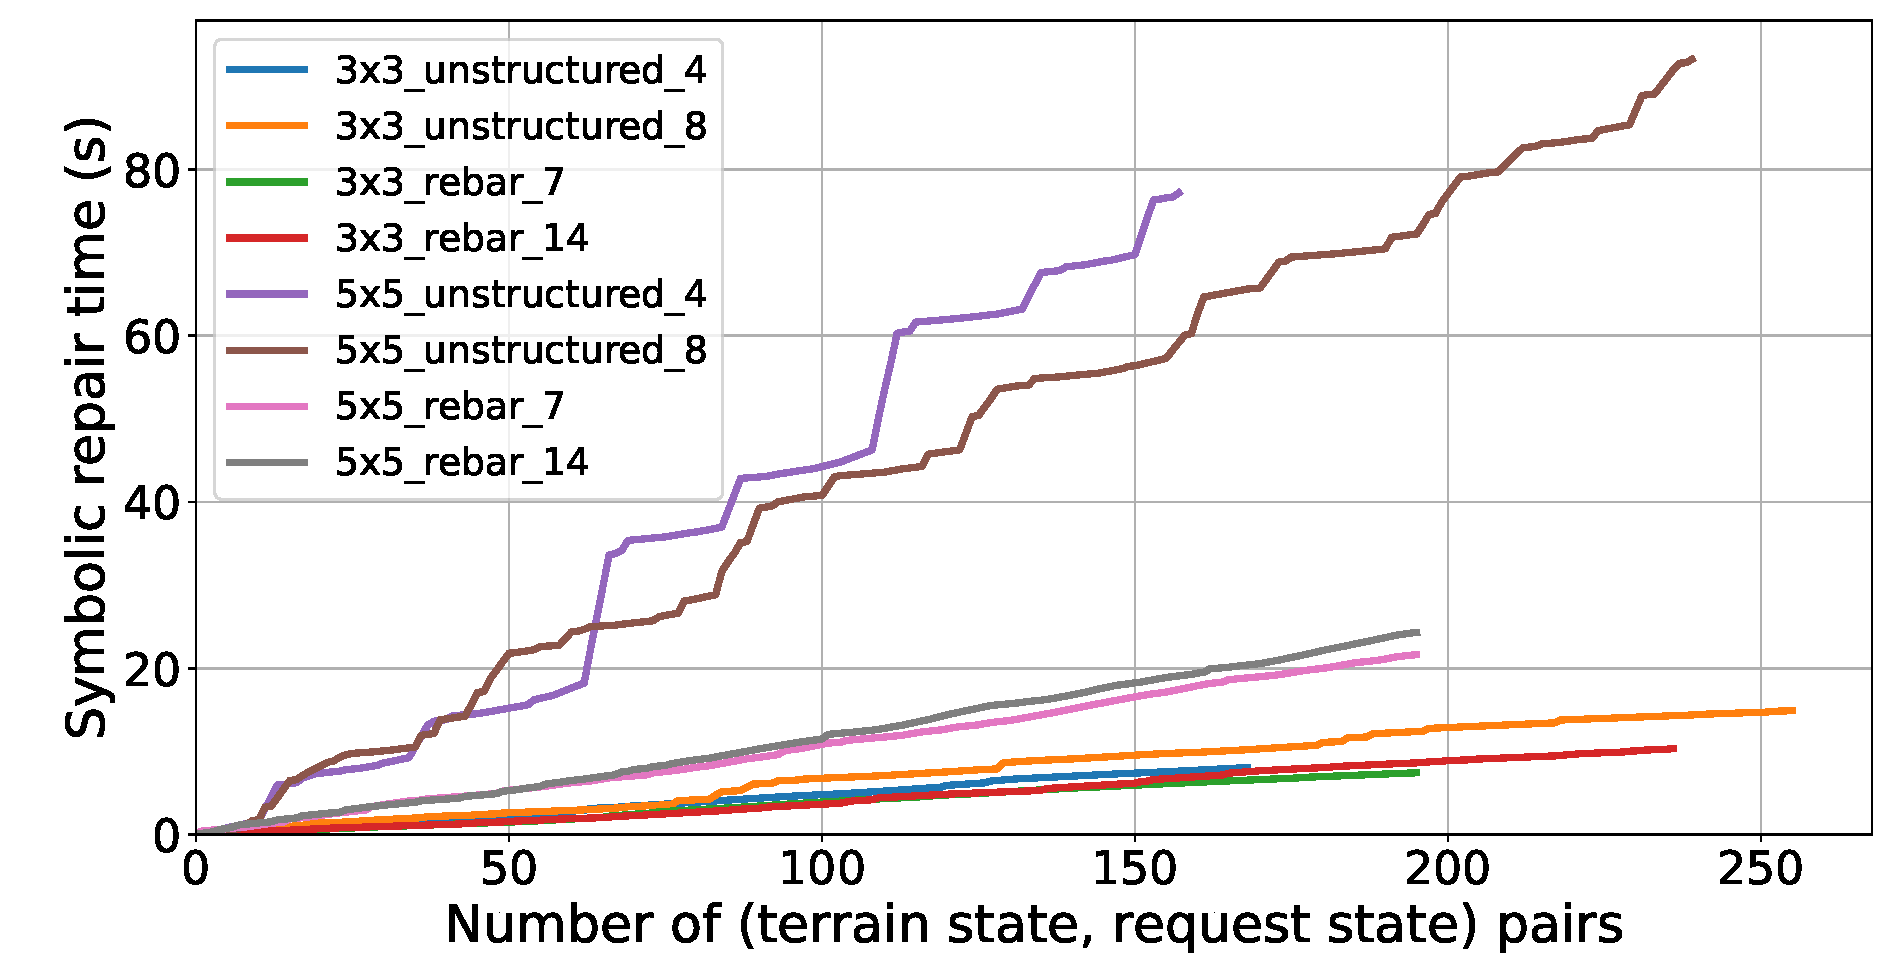
\includegraphics[width=\linewidth]{num_states_vs_repair_time.pdf}
    \caption{Offline symbolic-repair time versus the number of terrain--request state pairs for the $3\times 3$ and $5\times 5$ abstractions. Repair time grows approximately linearly in both cases; per state pair, the $5\times 5$ grid takes $478.1\%$ more time than the $3\times 3$ grid.}
    \label{fig:repair_vs_num_states}
\end{figure}

\begin{table*}
\centering
\small
    \caption{Online Gait-Fixed MICP Solving Time for Simulation}
    \setlength{\tabcolsep}{4pt}
     \begin{tabular*}{\linewidth}{@{\extracolsep{\fill}}cccccc}
         \hline
         \textbf{Scenario} & \textbf{Collision Avoidance} &
         \textbf{Binary Variables} &
         \textbf{Continuous Variables} &
         \textbf{Number of Polygons} &
         \textbf{Solve Time (s)}\\\hline
         Unstructured - 4 & No & 52 & 6583.5 & 6.5 & 0.37\\\hline
         Unstructured - 8 & Yes & \textcolor{red}{256} & 5166 & 2 & \textcolor{red}{2.65}\\
         & No & 69 & 7938 & 7.5 & 0.49\\\hline
         Rebar - 7& No & 70 & 7938 & 7.875 & 1.11\\
         \hline
         Rebar - 14 & No & 58 & 8142.75 & 6.25 & 1.09\\\hline
    \end{tabular*}
    \label{tab:micp_speed}
\end{table*}

\subsection{Offline Synthesis Results}
We evaluate the offline synthesis module for both \textit{Unstructured} and \textit{Rebar Terrain} scenarios by initializing the skill set with two trotting gaits ($2$ s and $3$ s). The inclusion of the longer-horizon trotting gait provides additional safer walking options from a practical standpoint. Prior to synthesis, we construct the set of possible terrain states $\inpstatesterrainexprposs$—assumed to be provided by the user—by systematically sweeping a local grid over the entire terrain map, based on the best available prior knowledge. The set of request states $\inpstatesrequestposs$ is defined as the top row of the local grid in the robot's facing direction, with the two corner cells also included to enable movement in diagonal directions.

% We briefly summarize the key offline synthesis statistics previously reported in \citep{zhou2025physically}. Specifically, the repair process was shown to successfully handle approximately $93.4\%$ of all terrain and request state pairs $(\inpstateterrain, \inpstaterequest) \in \inpstatesterrainexprposs \times \inpstatesrequestposs$. The remaining $6.6\%$ were unrepairable due to either unreachable request states caused by obstacles or physical infeasibility. Notably, the number of newly discovered skills was reduced by $71.6$–$97.6\%$ compared to checking the full space of all possible skills, each requiring the solution of a costly gait-free MICP. On average, generating a new locomotion gait via gait-free MICP took $27.23$ s, with a maximum time of $145.66$ s. These results demonstrate the effectiveness of the offline repair strategy in minimizing expensive MICP solves. For a full breakdown of synthesis time, number of symbolic states, and repair outcomes, please refer to \citep{zhou2025physically} (Table I).

Table~\ref{tab:offline_synthesis_time} reports 
\begin{enumerate*}[label=(\roman*),ref=\roman*]
    \item the number of terrain and request states pairs $(\inpstateterrain, \inpstaterequest) \in \inpstatesterrainexprposs \times \inpstatesrequestposs$, including both successful and total ones,
    \item the number of skills, 
    including the original,
    the newly discovered,
    and the total possible ones,
    and
    \item offline repair and feasibility checking times, including both from gait-fixed and gait-free MICP.
\end{enumerate*}
We first observe that the repair process successfully resolves $93.4\%$ of the terrain and request state pairs. The remaining cases are deemed unrepairable due to either unreachable request states caused by obstacles or inherent physical infeasibility. As highlighted in red, the number of newly discovered skills is reduced by $71.6$–$97.6\%$ compared to exhaustively checking all possible skills—each of which requires solving a computationally expensive gait-free MICP. On average, generating a new locomotion gait via gait-free MICP takes $27.23$ s, with a maximum of $145.66$ s. This demonstrates the effectiveness of offline repair in substantially reducing the number of costly gait-free MICP solves.


To investigate the scalability of offline repair,
we perform repair across various sizes of the terrain and request states.
As shown in
Fig.~\ref{fig:repair_vs_num_states},
the repair runtime grows linearly in the size of the terrain and request states for both $3\times 3$ and $5 \times 5$ grids.
While fewer terrain and request states handled offline reduce checked time, they may lead to more frequent unforeseen states during online execution.
%
Moreover, we note that
the slope of $5 \times 5$ cases in Fig.~\ref{fig:repair_vs_num_states}
are steeper than those of $3\times 3$
% because 
as a result of the increased state space.
% We further note that 
On average,
repair takes 478.1$\%$ more time for $5\times 5$ grids than $3\times 3$ for one terrain and request states pair.
% However, 
%
In practice, 
the perception range and the robot size limit the grid size, 
so we do not test beyond $5\times 5$ grids,
though the user can adjust the resolution.

\begin{figure*}[t]
    \centering
    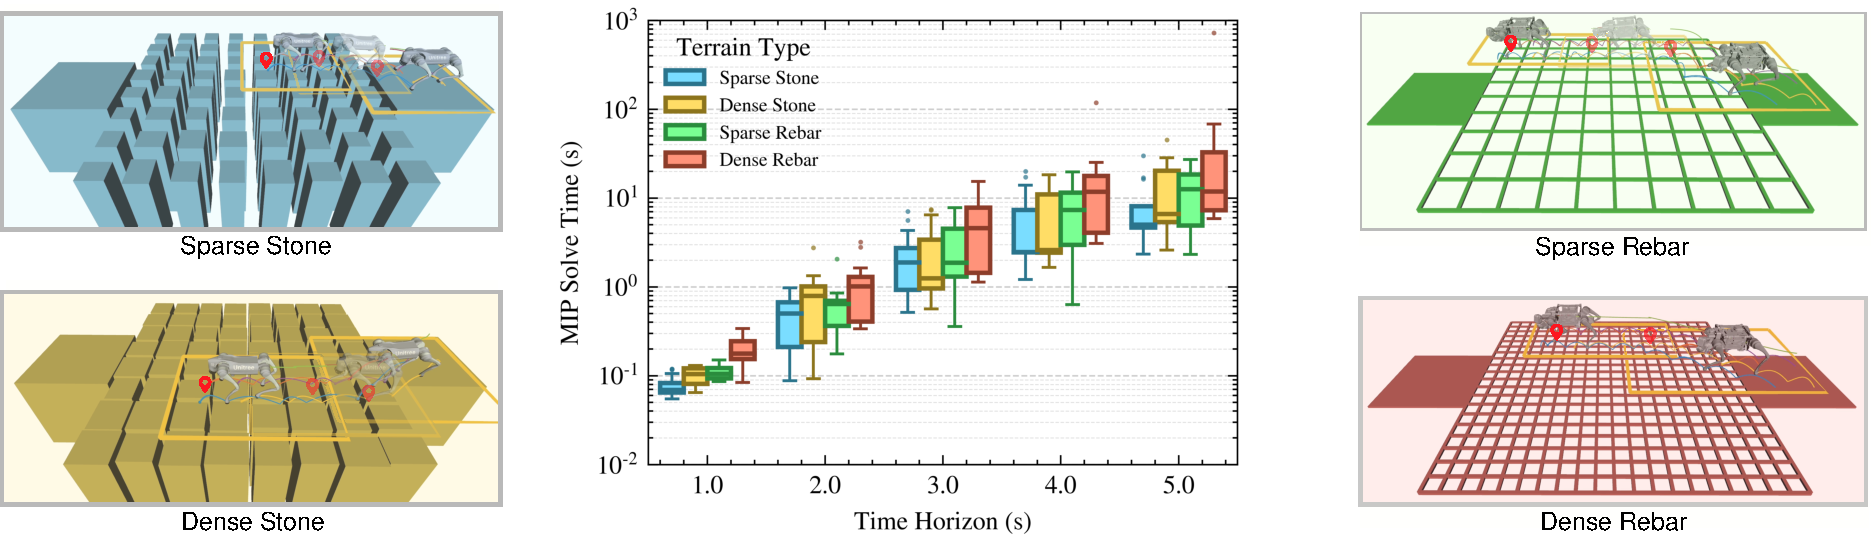
\includegraphics[width=\linewidth]{pure_mip_benchmark_box_plot.pdf}
    \caption{\revised{MIP solve time across four terrains---sparse stone (blue), dense stone (yellow), sparse rebar (green), dense rebar (red)---and horizons of $1$--$5$\,s, as box plots over $10$ seeded waypoints per scenario. In each terrain subfigure, selected traversal snapshots at planning horizons of $1$\,s (blue), $2$\,s (yellow), $4$\,s (green), and $5$\,s (red) are overlaid for visualization.}}
    \label{fig:pure_mip_benchmark}
\end{figure*}

\begin{figure}
    \centering
    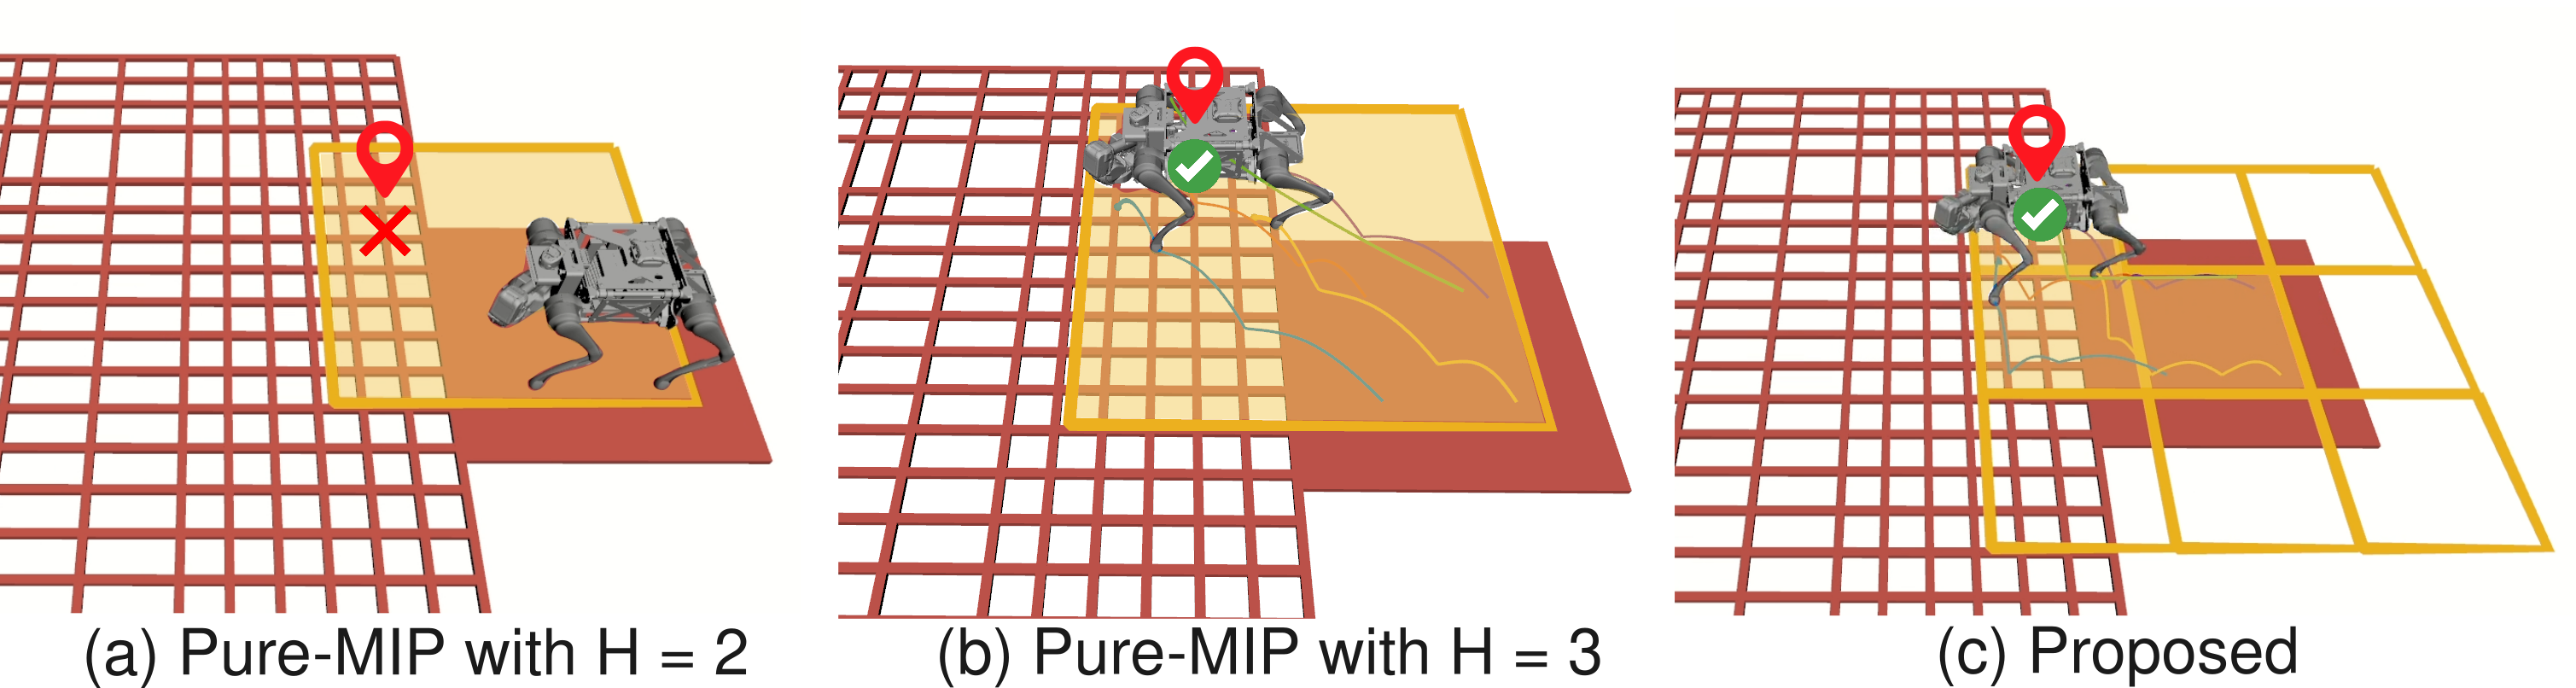
\includegraphics[width=\linewidth]{dense_rebar_comparison.png}
    \caption{\revised{Representative dense rebar trial after randomly removing terrains for benchmarking different baselines: (a) Pure-MIP with $H{=}2$ s; (b) Pure-MIP with $H{=}3$ s; (c) Proposed approach with $3\times 3$ grid.}}
    \label{fig:dense_rebar_comparison}
\end{figure}

\subsection{Online Execution Results}
Fig.~\ref{fig:online_terrains} presents snapshots of Go2 and Chotu navigating various terrains during online execution. The robot is tasked with reaching a global waypoint using a naive global shortest-path planner. At each step, the local waypoint is selected as the closest non-obstacle cell in the local grid map pointing toward the global target.

In Fig.~\ref{fig:online_terrains}(a), the robot traverses a sequence of terrain types including \textit{flat terrain}, \textit{dense stepping stone}, \textit{sparse stepping stone}, and \textit{gap}. Fig.~\ref{fig:online_terrains}(b) showcases a more complex maneuver involving all eight terrain types, including elevation changes, where the robot adaptively selects suitable locomotion gaits. Similarly, Figs.~\ref{fig:online_terrains}(c) and (d) illustrate Chotu traversing rebar terrains with 7 and 14 defined rebar types, respectively.
Notably, the robot utilizes newly discovered leaping gaits with short aerial phases to execute challenging transitions—such as moving from lower to higher elevations or crossing over gaps and \textit{extreme sparse} rebar segments, as demonstrated in Figs.~\ref{fig:online_terrains}(b) and(d).

Table \ref{tab:micp_speed} summarizes the average number of decision variables, terrain polygons, and solve time for each scenario, computed across all step transitions in a full locomotion run with the online gait-fixed MICP.
%\ye{[why the number of continuous variables has decimal digits?]}\ziyi{[The planner could choose adaptive gaits with different time horizons.]} \ye{[Ok, then we should provide some more info on how the average number is calculated. Is it based on 100 trials randomly selected or under certain trial conditions?]} \ziyi{[Rephrased this sentence. It's averaged only because each maneuver includes multiple transitions and solve MICP multiple times.]} \ye{[can we say "across all step transitions during one full locomotion run?"]\ziyi{Done}}
On average, the online gait-fixed MICP takes $430$ ms to solve the unstructured terrain cases and $1.1$ s for rebar cases when the collision avoidance is disabled. 
% the time horizon ranges from $1.5$ s to $3.0$ s, 
% depending on the chosen gait. 
The rebar scenarios exhibit $155.8\%$ longer solve times due to their overlapping, skewed rebar arrangement, and a larger number of terrain polygons. 
Additionally, 
enabling 
collision avoidance (necessary for \textit{Unstructured - 8} case to handle the elevation change) 
increases the number of binary variables
by $271.0\%$, 
increasing the solve time 
% to $2.65$ s.
by $440.8\%$
(highlighted in red).

\revised{\subsection{Runtime Repair Case Study}\label{sec:runtime_repair_case_study}
As a case study to demonstrate the framework's capability to handle unforeseen terrains and online failures, we highlight the following run-time scenarios that trigger runtime repair or re-synthesis.

\subsubsection{Unforeseen Terrain States}
With limited prior knowledge of the global terrain map, the terrain states provided during offline synthesis may be insufficient when encountering new terrain configurations. Fig.~\ref{fig:online_repair} illustrates this in an \textit{Unstructured - 4 types} scenario with a $3 \times 3$ grid size, where terrain states involving \textit{gap} terrain are deliberately excluded from the offline phase. When the robot reaches a new terrain state that contains a \textit{gap}, runtime repair is triggered for the current terrain and request states. A new skill with a leaping gait is generated to successfully cross the gap. The runtime repair takes $12.36$\,s in total, of which the symbolic-repair stage accounts for $0.18$\,s and the gait-free MICP for the new leaping gait accounts for $12.18$\,s---confirming that the dominant cost lies in the dynamic-feasibility check, not the symbolic search.

\subsubsection{Solving Failure}
Another common runtime failure arises from MICP solving failures. Due to discrepancies between the predefined polygons used during offline synthesis and the actual online terrains---such as variations in shape and size---a skill deemed feasible offline may become infeasible when executed online, even if classified under the same symbolic transition. The detours shown in Fig.~\ref{fig:online_terrains}(c) and (d) illustrate the re-synthesis process triggered by solving failures in the 7-type and 14-type rebar cases. Solving failures occur more frequently in the rebar scenarios than in the unstructured ones, due to the higher uncertainty in the shapes and sizes of online rebar polygons. Re-synthesis takes $0.11$\,s and $0.07$\,s respectively for the two cases. Neither case triggers full runtime repair, because the existing skill set suffices to navigate to the goal under the failed transition.}

\subsection{Benchmark: Pure-MIP Planner}
To evaluate how the symbolic-continuous planner separation benefits the overall planning framework, we benchmark our method against \textit{pure-MIP} approaches, where we implement a planner to evaluate how computation time scales with the planning horizon and terrain complexity. \revised{The pure-MIP approach can also be treated as an ablation study for the symbolic planning.} Specifically, we examine five planning horizons ranging from $1$ s to $5$ s. In addition, we vary the terrain types by considering sparse stepping stones (0.15 m spacing), dense stepping stones (0.05 m spacing), sparse rebar (0.3 m spacing), and dense rebar (0.15 m spacing), as illustrated in Fig.~\ref{fig:pure_mip_benchmark} with specific colors.

\revised{To make the comparison precise: the pure-MIP baseline uses the \emph{same} convex relaxations of the dynamics (Eq.~(\ref{eq:dynamics})), the \emph{same} linearized friction-cone and fixed-Jacobian kinematic constraints, and the \emph{same} cost weights as our online gait-fixed MICP. The only differences are (i) the planner solves a single long-horizon gait-fixed MICP without symbolic-level decomposition, and (ii) the local planning region is expanded to encompass all terrain polygons within the horizon-induced reachable distance, rather than being limited to the cells adjacent to a symbolic transition. The same Gurobi solver and settings are used in both cases.}

\revised{The pure-MIP planner uses an \emph{adaptive} local region whose maximum size scales with the planning horizon $H$ (in seconds): along each axis the region spans up to $\textrm{gs} + (\textrm{gs}/2)\cdot H$, where $\textrm{gs}$ is the symbolic-cell grid spacing, with a floor of $1.5\,\textrm{gs}$ corresponding to the $H{=}1$\,s setting. So the $H{=}2$\,s column reads as a like-for-like comparison for an equivalent two-cell transition footprint, while each additional second of horizon adds half a cell of reach. As shown in Fig.~\ref{fig:pure_mip_benchmark}, the region further shrinks when the goal lies within the maximum range, avoiding redundant incorporation of terrain polygons in each MIP solve. 
% so the per-MIP foothold set always stays proportional to the distance the gait can traverse in one solve. 
In contrast, our proposed planner always plans against a fixed $3{\times}3$ symbolic grid centered on the robot, decoupling the per-MIP problem size from the total traversal distance. We omit the gait-free MICP from the benchmark because its solve time becomes prohibitively long once $H>2$\,s; the locomotion gait is repeated cyclically on a $1$\,s trotting pattern, and the planner receives a global waypoint and incrementally computes local waypoints as in the proposed framework.}

\revised{Fig.~\ref{fig:pure_mip_benchmark} also reports the per-MIP solve time as box plots aggregated over $10$ randomly sampled waypoints per scenario. Within the same terrain, the solve time grows almost exponentially with the horizon, and the dense variants consistently take longer than their sparse counterparts because more terrain polygons enter the MIP. The $H{=}1$\,s setting is too myopic to commit to scenarios that require multi-step planning, while $H\ge4$\,s pushes the median solve into multiple seconds even for the easier scenarios. The $H{=}2$\,s and $H{=}3$\,s horizons sit on the knee of this trade-off curve, balancing optimality and per-step compute, and we therefore adopt them as the two reference pure-MIP configurations for the end-to-end benchmark below.}

\revised{To assess closed-loop behavior beyond a per-MIP solve time, we run an end-to-end comparison on the dense rebar scenario, where the pure-MIP planner is most stressed. For each method, we dispatch $10$ seeded random waypoints; between trials the robot is reset back to the launch pose, and we randomly remove a fraction of the rebar polygons as shown in Fig.~\ref{fig:dense_rebar_comparison} to add randomness and make the scenario more challenging. Identical random seeds across methods ensure all baselines see the byte-for-byte same waypoints and terrain, so any difference in outcome reflects the planner alone. Fig.~\ref{fig:dense_rebar_comparison} also shows one representative instance on which the pure-MIP planner with short horizons (i.e., 1 or 2 s) stalls---the planning region is too limited for the solver to discover a feasible routing path% the resulting foothold pattern forces the MIP to at most backtrack within its local region and the planner has no mechanism to deliberate at the symbolic level about which neighboring cell to attempt next
, whereas the proposed planner routes through a sequence of cells.}

\revised{Table~\ref{tab:pure_mip_benchmark} reports the success rate, mean traversal time of successful trials, and the mean per-module active computation per trial---broken down into MIP transition solving, the pre-flight MIP feasibility check (FC), reactive synthesis (strategy query plus strategy reload), and runtime repair (online specification regeneration). In this scenario, the proposed planner attains $90\%$ success rate with $18.5$\,s mean traversal time, matching the $H{=}3$\,s pure-MIP success rate ($90\%$) at roughly three quarters of the traversal time and at less than half the MIP transition cost ($5.26$\,s vs.\ $11.54$\,s per trial). The shorter $H{=}2$\,s pure-MIP setting reaches only $60\%$, indicating that its horizon is too myopic to recover from the gaps. The two ablation rows confirm the value of the online additions introduced in this work: disabling the FC drops the success rate substantially in both planners ($60\%\rightarrow20\%$ for pure-MIP at $H{=}2$\,s and $90\%\rightarrow60\%$ for the proposed planner); disabling the delay-aware coordination (DAC) preserves the $90\%$ success rate of the proposed planner but inflates the mean traversal time from $18.5$\,s to $23.4$\,s, because each symbolic transition now must wait for the previous trajectory to be fully tracked before the next MIP solve can start.}

\begin{table*}[t]
\centering
\caption{\revised{End-to-end benchmark on the dense rebar scenario ($10$ seeded waypoints, identical seed and terrain across methods, with randomly removed rebars per trial to add randomness). Traversal time and per-module times are mean values computed over successful trials only. Reactive synthesis combines the per-step strategy query and the per-spec-switch strategy reload. Dashes denote modules that do not exist in the corresponding method or are disabled by the ablation.}}
\label{tab:pure_mip_benchmark}
\setlength{\tabcolsep}{4pt}
{\color{blue}
\begin{tabular}{lcccccc}
\hline
\textbf{Method} & \textbf{Success} & \textbf{Traversal} & \textbf{MIP trans.} & \textbf{MIP feas.} & \textbf{Reactive synth.} & \textbf{Runtime repair} \\
 & \textbf{rate} & \textbf{time (s)} & \textbf{solving (s)} & \textbf{check (s)} & \textbf{(query + load, s)} & \textbf{(s)} \\
\hline
Pure MIP ($H{=}2$\,s)                              & 60\% (6/10) & 14.76 &  3.04 & 0.21 & --   & --   \\
Pure MIP ($H{=}3$\,s)                              & 90\% (9/10) & 24.73 & 11.54 & 0.19 & --   & --   \\
Pure MIP ($H{=}2$\,s), no FC        & 20\% (2/10) &  9.00 &  1.38 & --   & --   & --   \\
Pure MIP ($H{=}3$\,s), no FC        & 40\% (4/10) & 14.23 &  5.17 & --   & --   & --   \\
\hline
Proposed                                           & 90\% (9/10) & 18.48 &  5.26 & 0.19 & 0.29 & 0.03 \\
Proposed, no FC                     & 60\% (6/10) & 20.08 &  5.85 & --   & 0.33 & 0.05 \\
Proposed, no DAC & 90\% (9/10) & 23.43 &  5.11 & 0.27 & 0.28 & 0.04 \\
\hline
\end{tabular}
}
\end{table*}

\subsection{Preliminary Study: Yaw Command Extension}\label{sec:extension}
\begin{figure}
    \centering
    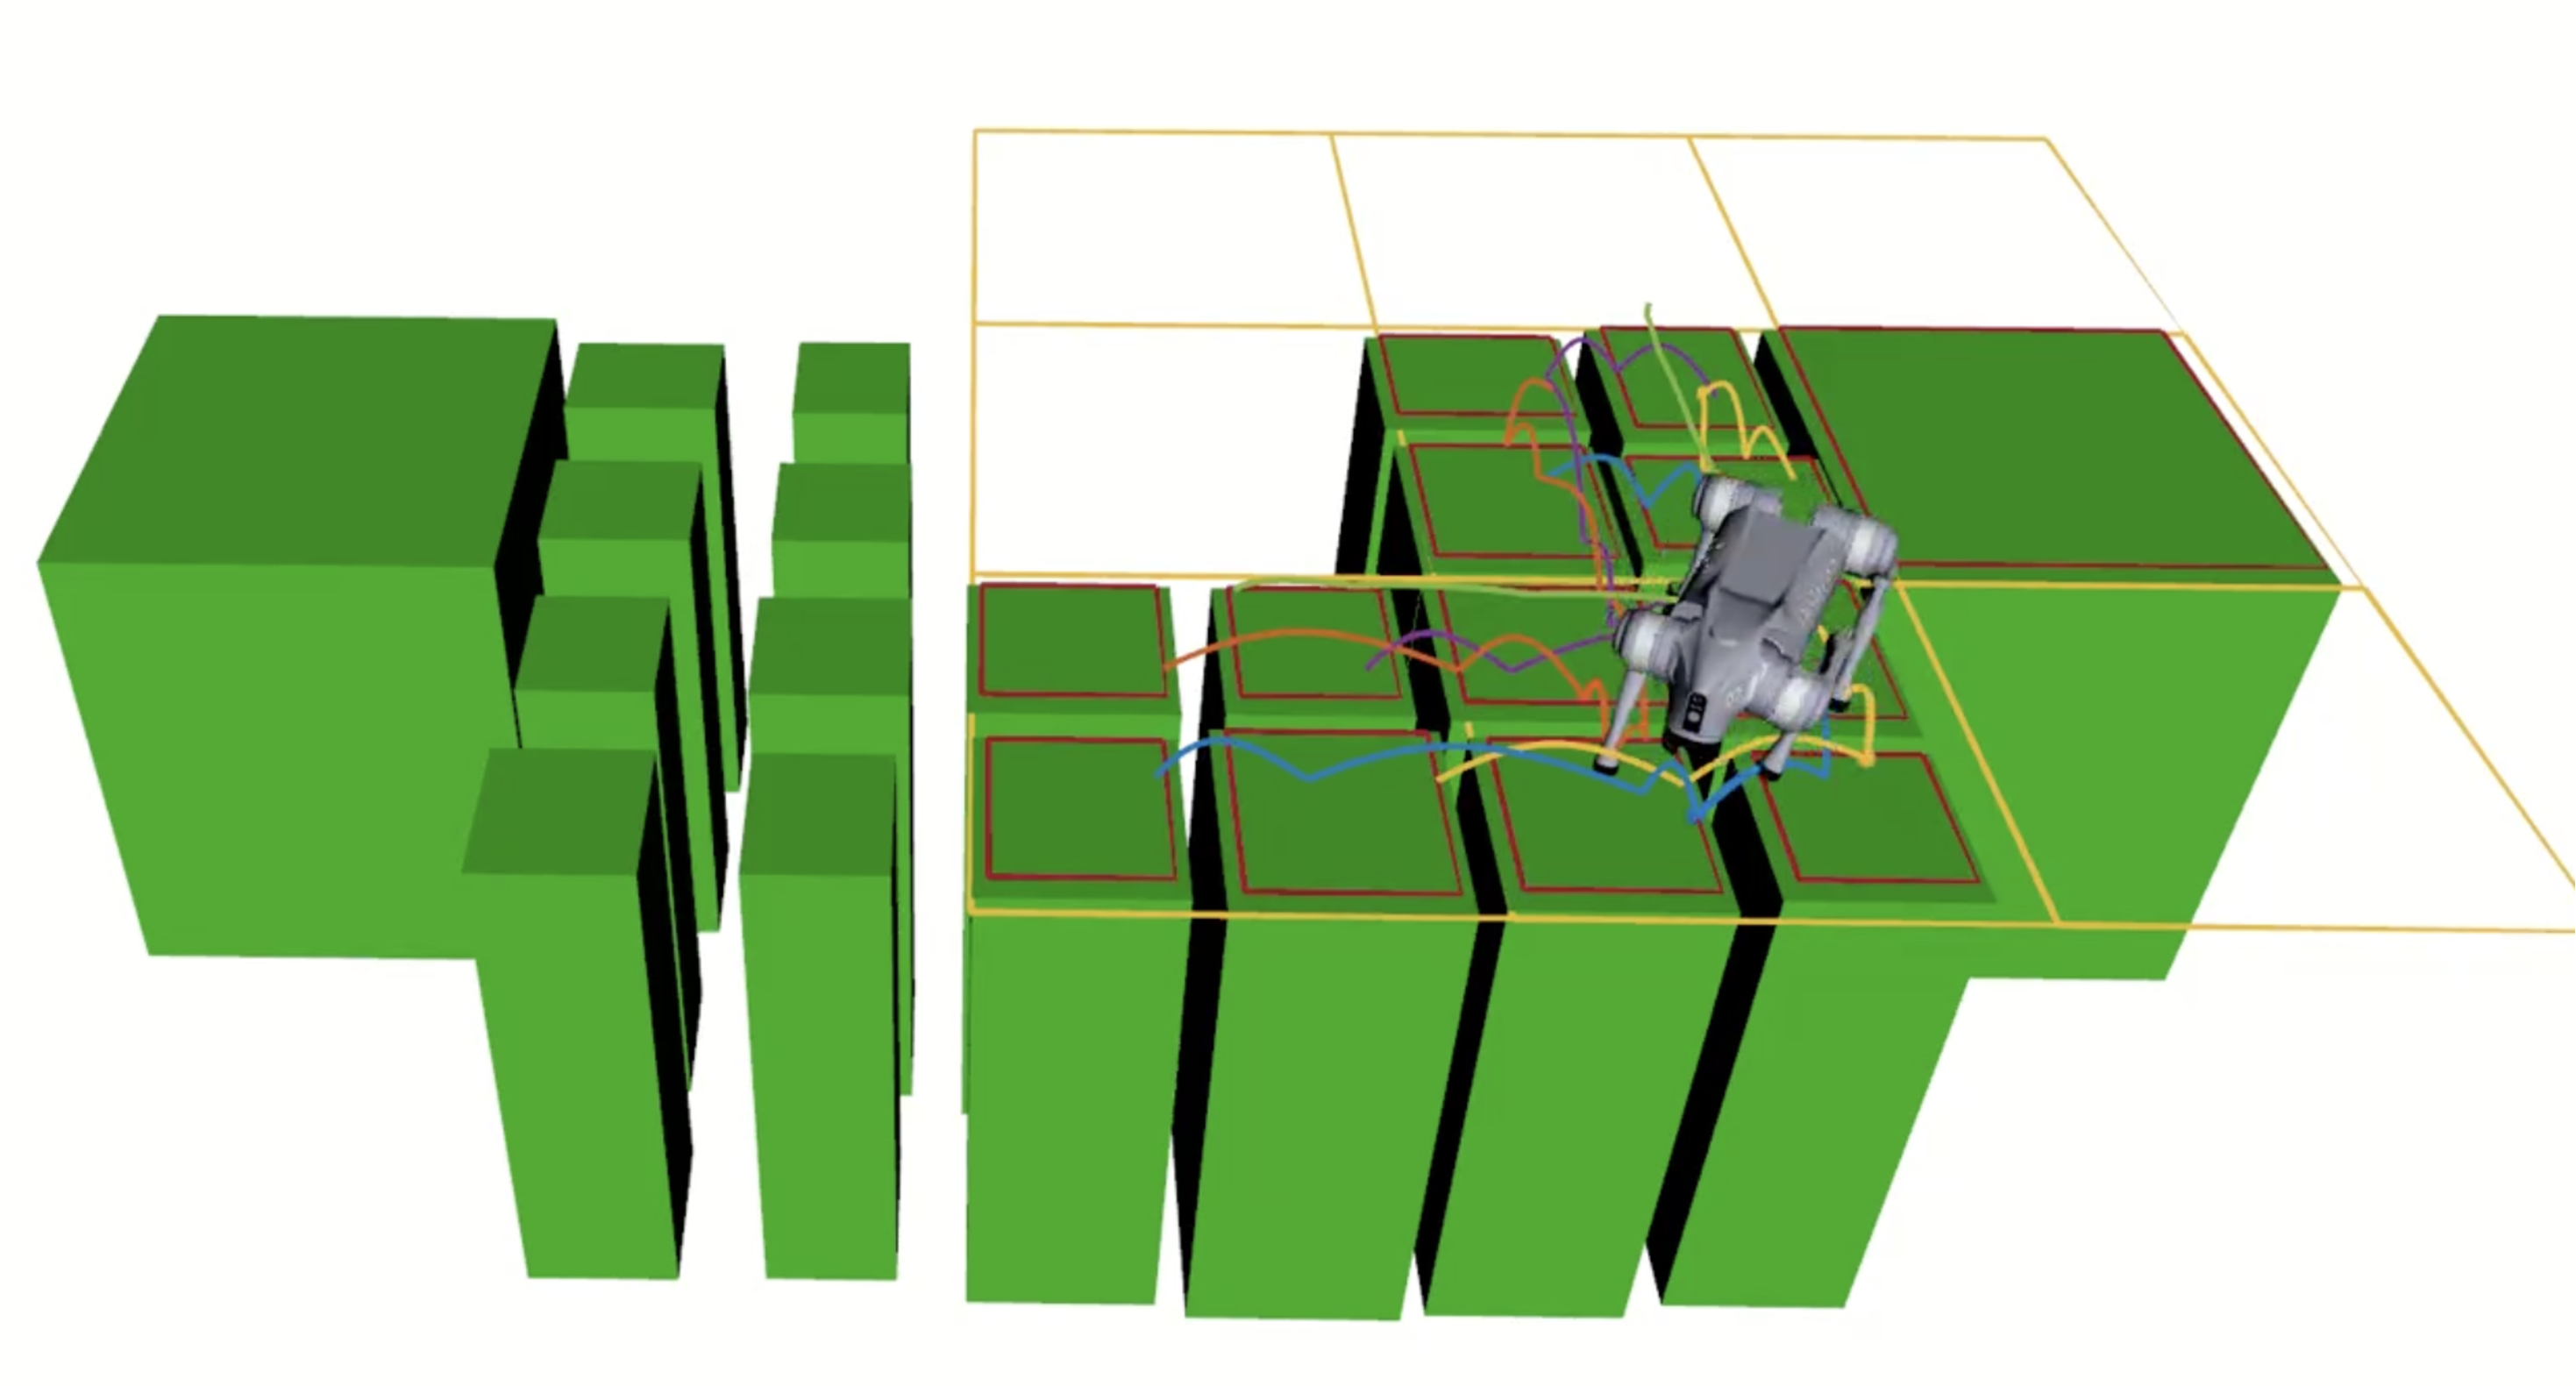
\includegraphics[width=\linewidth]{yaw_extension_demo.pdf}
    \caption{Demonstration of the robot executing multiple turning behaviors to continuously progress toward the global waypoint on terrain arranged in a zig-zag pattern.}
    \label{fig:yaw_extension}
\end{figure}
\revised{This subsection demonstrates that the proposed framework can be extended to non-zero yaw waypoints in principle, but we report the result as a \emph{preliminary feasibility study} only. We do not claim a full demonstration of generalizability of any angular movements. Specifically: (i) the symbolic abstraction in Sec.~\ref{sec:preliminaries_abstraction} grows combinatorially when yaw is added as a discretized input, and we have not characterized how the manager and symbolic-repair scaling numbers reported in Sec.~\ref{sec:experiments} change with yaw discretization; (ii) the angular-momentum coupling neglected by the convex-dynamics simplification in Eq.~(\ref{eq:dynamics}) becomes more relevant once yaw is treated as a planned variable, especially for fast turns; (iii) we report simulation results only---no hardware deployment of the yaw extension.}

In the previous examples, we assume that the yaw angle of the robot base is fixed to simplify the problem. However, the robot's physical capability to traverse terrains largely depends on the base orientation. For instance, performing a forward jump onto a high terrain is different from a sideway jump, in terms of both leg kinematics and dynamics.
Therefore, to demonstrate the framework's modularity, we provide a preliminary extension to the existing abstraction of the robot state to allow yaw variation.

Specifically, the robot inputs are now defined as
$\inpcen \coloneqq 
\{\var_x \mid x \in \xcells\} \cup 
\{\var_y \mid y \in \ycells\} \cup \{\var_{yaw} \mid yaw \in \mathcal{W}\}$, where we define a new set of yaw angles $\mathcal{W} \coloneqq \{-180 \degree, -90 \degree, 0 \degree, 90 \degree, 180 \degree\}$. Note that, a finer discretization of the yaw angles can be defined as needed.
Similarly, the request inputs are defined as 
$\inprequest \coloneqq
\{\var_x^\textrm{req} \mid x \in \xcells\} \cup 
\{\var_y^\textrm{req} \mid y \in \ycells\} \cup \{\var_{yaw}^\textrm{req} \mid yaw \in \mathcal{W}\}$. The robot and the request input can be further divided into translational 
$\inpcentrans, \inprequesttrans$ and rotational parts $\inpcenorien, \inprequestorien$, where the translational ones contain the $x$ and $y$ states and the orientational ones contain the $yaw$ state.

The skill is further divided into translational and rotational skills. A translational skill $\skill_{\textrm{trans}} \in \out_{\textrm{trans}}$
consists of 
sets of preconditions $\skillpretrans \subseteq \inpstatescen \times \inpstatesterrain$ that include the full robot state, and 
% a set of 
translational-only postconditions $\skillposttrans \subseteq \inpstatescen^{\textrm{trans}}$. A rotational skill in place $\skill_{\textrm{orien}} \in \out_{\textrm{orien}}$ consists of sets of rotational-only preconditions $\skillpreorien \subseteq \inpstatescen^{\textrm{orien}}$ and postconditions $\skillpostorien \subseteq \inpstatescen^{\textrm{orien}}$. The terrain state can also be incorporated when generating rotational skills, particularly for terrains that pose challenges for turning. However, we omit this in our current implementation for simplicity. The specification encoding then follows the same procedure as described in Sec.~\ref{sec:spec_gen}, based on each skill's precondition and postcondition. The hard constraints remain unchanged, except that translational and rotational ones are defined separately to ensure the corresponding states remain unchanged when no skill is selected.

To demonstrate the resulting maneuver, we construct a scenario with multiple dense and sparse stepping stones arranged in an overall zig-zag pattern, requiring several turning behaviors. Although sideways movement skills are feasible, we manually exclude them before synthesis to highlight yaw adjustments controlled by the rotational skills. As shown in Fig.~\ref{fig:yaw_extension}, the robot executes multiple turns to continuously progress towards the global waypoint. More complex coupled translational and rotational behaviors can also be defined by modifying the preconditions and postconditions associated with each skill.

% \subsubsection{Diagonal Movement}\label{sec:extension_diag}


